%% LyX 2.0.4 created this file.  For more info, see http://www.lyx.org/.
%% Do not edit unless you really know what you are doing.
\documentclass[english]{beamer}
\usepackage{mathpazo}
\usepackage{helvet}
\usepackage[]{fontenc}
\usepackage[latin9]{inputenc}
\setcounter{secnumdepth}{3}
\setcounter{tocdepth}{3}
\setlength{\parskip}{\medskipamount}
\setlength{\parindent}{0pt}
\usepackage{graphicx}

\makeatletter

%%%%%%%%%%%%%%%%%%%%%%%%%%%%%% LyX specific LaTeX commands.
\providecommand{\LyX}{L\kern-.1667em\lower.25em\hbox{Y}\kern-.125emX\@}

%%%%%%%%%%%%%%%%%%%%%%%%%%%%%% Textclass specific LaTeX commands.
 % this default might be overridden by plain title style
 \newcommand\makebeamertitle{\frame{\maketitle}}%
 \AtBeginDocument{
   \let\origtableofcontents=\tableofcontents
   \def\tableofcontents{\@ifnextchar[{\origtableofcontents}{\gobbletableofcontents}}
   \def\gobbletableofcontents#1{\origtableofcontents}
 }
 \def\lyxframeend{} % In case there is a superfluous frame end
 \long\def\lyxframe#1{\@lyxframe#1\@lyxframestop}%
 \def\@lyxframe{\@ifnextchar<{\@@lyxframe}{\@@lyxframe<*>}}%
 \def\@@lyxframe<#1>{\@ifnextchar[{\@@@lyxframe<#1>}{\@@@lyxframe<#1>[]}}
 \def\@@@lyxframe<#1>[{\@ifnextchar<{\@@@@@lyxframe<#1>[}{\@@@@lyxframe<#1>[<*>][}}
 \def\@@@@@lyxframe<#1>[#2]{\@ifnextchar[{\@@@@lyxframe<#1>[#2]}{\@@@@lyxframe<#1>[#2][]}}
 \long\def\@@@@lyxframe<#1>[#2][#3]#4\@lyxframestop#5\lyxframeend{%
   \frame<#1>[#2][#3]{\frametitle{#4}#5}}
 \newenvironment{lyxcode}
   {\par\begin{list}{}{
     \setlength{\rightmargin}{\leftmargin}
     \setlength{\listparindent}{0pt}% needed for AMS classes
     \raggedright
     \setlength{\itemsep}{0pt}
     \setlength{\parsep}{0pt}
     \normalfont\ttfamily}%
    \def\{{\char`\{}
    \def\}{\char`\}}
    \def\textasciitilde{\char`\~}
    \item[]}
   {\end{list}}
 \long\def\lyxplainframe#1{\@lyxplainframe#1\@lyxframestop}%
 \def\@lyxplainframe{\@ifnextchar<{\@@lyxplainframe}{\@@lyxplainframe<*>}}%
 \long\def\@@lyxplainframe<#1>#2\@lyxframestop#3\lyxframeend{%
   \frame<#1>[plain]{\frametitle{#2}#3}}

%%%%%%%%%%%%%%%%%%%%%%%%%%%%%% User specified LaTeX commands.
%\usepackage{beamerthemesplit}
\usepackage{beamerthemeBerlin}
\newcommand{\ds}{\displaystyle}

\makeatother

\usepackage{babel}
\begin{document}

\title{Literate programming, Matlab \&\\
finite element method}


\author{David Stewart}

\makebeamertitle

\lyxframeend{}


\lyxframeend{}\section{Introduction}


\lyxframeend{}\lyxframe{Literate programming}
\begin{itemize}
\item Originally developed by Donald Knuth while creating \TeX
\item Combines code (e.g., Pascal) and documentation (e.g., \TeX/\LaTeX)
\item Knuth's system was called WEB
\end{itemize}
\noindent \begin{center}
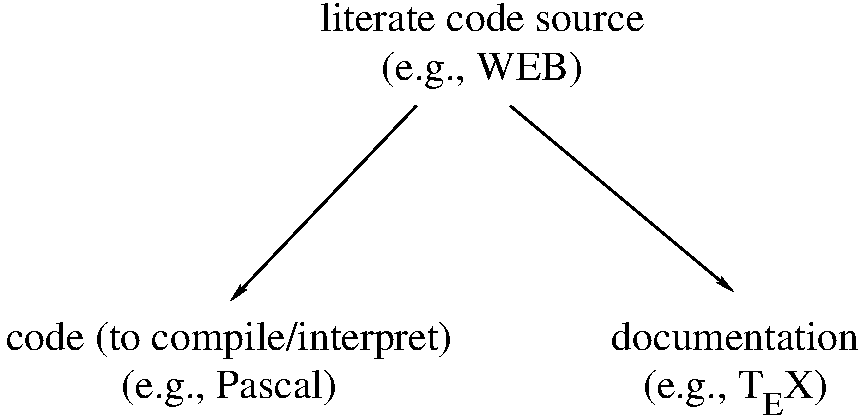
\includegraphics[width=5cm]{WEB-intro}
\par\end{center}


\lyxframeend{}


\lyxframeend{}\lyxframe{NoWeb}
\begin{itemize}
\item NoWeb is a simple version of this designed for any kind of source
code
\item Unlike WEB, there is no prettyprinting of the source code
\item Documentation is in \TeX/\LaTeX
\end{itemize}

\lyxframeend{}


\lyxframeend{}\lyxframe{What NoWeb looks like}

Source (NoWeb):
\begin{lyxcode}
For~the~PDE~\$-\textbackslash{}Delta~u=f(\textbackslash{}mathbf\{x\})\$~with

\$f(\textbackslash{}mathbf\{x\})=x\_\{1\}\textasciicircum{}\{2\}\textbackslash{},\textbackslash{}exp(x\_\{2\})\$,~we~use:

\textless{}\textless{}pde-struct-eg\textgreater{}\textgreater{}=~

pde~=~struct('coeffs',@(x)diag({[}0,1,1{]}),~...

~~~~~~~~~'rhs',@(x){[}x(1)\textasciicircum{}2{*}exp(x(2));0;0{]},'order',1)~

@~
\end{lyxcode}

\lyxframeend{}


\lyxframeend{}\lyxplainframe{}

What is looks like in the documentation:

\noindent \begin{center}
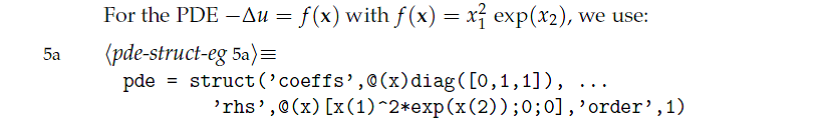
\includegraphics[width=1\textwidth]{sample-noweb}
\par\end{center}

In the code:
\begin{lyxcode}
pde~=~struct('coeffs',@(x)diag({[}0,1,1{]}),~...

~~~~~~~~~'rhs',@(x){[}x(1)\textasciicircum{}2{*}exp(x(2));0;0{]},'order',1)
\end{lyxcode}

\lyxframeend{}


\lyxframeend{}\lyxframe{More Noweb\ldots{}}

The basic syntax for the chunks of code is
\begin{lyxcode}
\textless{}\textless{}name-of-code\textgreater{}\textgreater{}=

code~chunk~goes~here

it~can~go~for~many~lines

but~it~ends~with~``@''

@
\end{lyxcode}
Actually ``@'' indicates the start of normal \LaTeX. You can have
several different chunks one after the other:
\begin{lyxcode}
\textless{}\textless{}chunk1\textgreater{}\textgreater{}=

This~is~chunk~1.

\textless{}\textless{}chunk2\textgreater{}\textgreater{}=

This~is~chunk~2.

@
\end{lyxcode}

\lyxframeend{}


\lyxframeend{}\lyxplainframe{}

Chunks can refer to other chunks.
\begin{lyxcode}
\textless{}\textless{}my-code.txt\textgreater{}\textgreater{}=

This~is~a~collection~of~chunks,~strung~together.

1st:~\textless{}\textless{}chunk1\textgreater{}\textgreater{}

2nd:~\textless{}\textless{}chunk2\textgreater{}\textgreater{}

@
\end{lyxcode}
If a chunk is ``defined'' multiple times, just concatenate the chunks
to form one large chunk:
\begin{lyxcode}
\textless{}\textless{}chunk3\textgreater{}\textgreater{}=

This~is~yet~another~chunk.

\textless{}\textless{}my-code.txt\textgreater{}\textgreater{}=

3rd:~\textless{}\textless{}chunk3\textgreater{}\textgreater{}

@
\end{lyxcode}
To generate code ``\texttt{chunks}'' from NoWeb file:Note that ``\texttt{my-code.txt}''
is the name of the root code chunk that is generated. A NoWeb file
can have many root chunks
\begin{lyxcode}
notangle~-Rmy-code.txt~source-file.nw~\textgreater{}~my-code.txt
\end{lyxcode}

\lyxframeend{}


\lyxframeend{}\lyxframe{Using with \LyX{}}

\LyX{} is a WYSIWYM \LaTeX-based editor.

\LyX{} has a large number of different styles (all from \LaTeX)
with convenient ways of handling cross-references, indexes, bibliographies,
structured documents, graphics, and can provide output in multiple
formats (DVI, PS, PDF, text, \LaTeX, OpenDocument) and NoWeb. 

The NoWeb export option produces a ``\texttt{.nw}'' file.


\lyxframeend{}


\lyxframeend{}\lyxframe{Pros \& Cons of literate programming}

\textbf{Pros:}
\begin{itemize}
\item Documentation and code are together.
\item Recursive use of code chunks encourages a top-down (``stepwise refinement'')
method of software development.
\item Not only can you have the formulas with the code, but also the \emph{derivation}
of the formulas can be kept with the code.
\item Graphics can be included in the documentation easily (unlike documentation
generated from source code).
\item There is a single source file (for everything!)
\end{itemize}

\lyxframeend{}


\lyxframeend{}\lyxplainframe{}

\textbf{Cons:}
\begin{itemize}
\item The run-debug-edit cycle is more complex.
\item Recursive use of code chunks encourages a top-down (``stepwise refinement'')
method of software development.
\item The documents tend to be rather large.
\item There is more work involved.
\item Not suitable for very large scale software development.
\end{itemize}

\lyxframeend{}


\lyxframeend{}\lyxframe{Pros and Cons of NoWeb}

\textbf{Pros:}
\begin{itemize}
\item Language independent --- can include scripts, Makefiles, and text
files for data or output
\item Simple syntax
\item Integrated into \LyX
\item Multi-platform (Unix/Linux, Mac, Windows under Cygwin)
\end{itemize}
\textbf{Cons:}
\begin{itemize}
\item Not maintained
\item Main implementation is based on the Icon programming language
\item Installation could be simpler
\item Does not allow underscore ``\_'' in chunk/file names
\end{itemize}

\lyxframeend{}


\lyxframeend{}\lyxframe{Tricks to make things easier}

Scripts and Makefiles can reduce the effort needed to use NoWeb: Makefiles
can be generated in NoWeb that will create all files desired from
the NoWeb file:
\begin{lyxcode}
notangle~-t8~-RMakefile~my-noweb-file.nw~\textgreater{}~Makefile

make~all
\end{lyxcode}
You need to add some items to your NoWeb file to do this. For each
root chunk for a file, add a \texttt{filelist} entry (only needed
once for each file):
\begin{lyxcode}
\textless{}\textless{}filelist\textgreater{}\textgreater{}=

new-file.txt~\textbackslash{}

\textless{}\textless{}new-file.txt\textgreater{}\textgreater{}=

....

@
\end{lyxcode}

\lyxframeend{}


\lyxframeend{}\lyxplainframe{}

A \texttt{Makefile} should be included:
\begin{lyxcode}
\textless{}\textless{}Makefile\textgreater{}\textgreater{}=

files1~=~\textless{}\textless{}filelist\textgreater{}\textgreater{}

files2~=~my-noweb-file.tex~filelist

files~=~\$(files1)~\$(files2)

source~=~pde-code.nw

all:~\$(files)

\$(files):~\$(source)

	~~~~notangle~-R\$@~\$(source)~\textgreater{}~\$@

my-noweb-file.tex:~\$(source)

	~~~~noweave~-delay~-index~\$(source)~\textgreater{}~\$@

@
\end{lyxcode}

\lyxframeend{}
\end{document}
